% ------------------------------------------------------------------------ %
% !TEX encoding = UTF-8 Unicode
% !TEX TS-program = pdflatex
% !TEX root = ../Tesi.tex
% !TEX spellcheck = it-IT
% ------------------------------------------------------------------------ %
%
% ------------------------------------------------------------------------ %
% 	NOME CAPITOLO
% ------------------------------------------------------------------------ %
%
\chapter{Experimental Results}
%
\label{cap:results}
%
\section{Experimental Testbed}
\subsection{Indoor Environment}
\subsection{Smartphones}
\subsection{WSN prototype}
\subsection{Back-end}
\section{Automatic Nodes Deployment Results}
Presented experimental results are initially focused on the usability of the tool, testing the ability to provide a solution in a reasonable time. Then, the performances of the model have been evaluated, in terms of localization accuracy through realistic indoor environment experiments, and in terms of cost-effectiveness of the suggested deployments.

\subsection{Computational Experience}\label{subsec:comp_res}
The tool has been been evaluated running several different configurations. Every test reported in this section has been executed with a spatial resolution of the floor plan equal to 1 meter.  A first analysis can be done on the execution times of the proposed solution. Although the execution time can be tuned by the parameter $R_{max}$, which represent the maximum number of restarts of the VNS algorithm, an idea on the order of magnitude is given by Figure~\ref{fig:time}, where the time is represented as a function of the floorplan dimension. 
\begin{figure}[h!tb]
\centering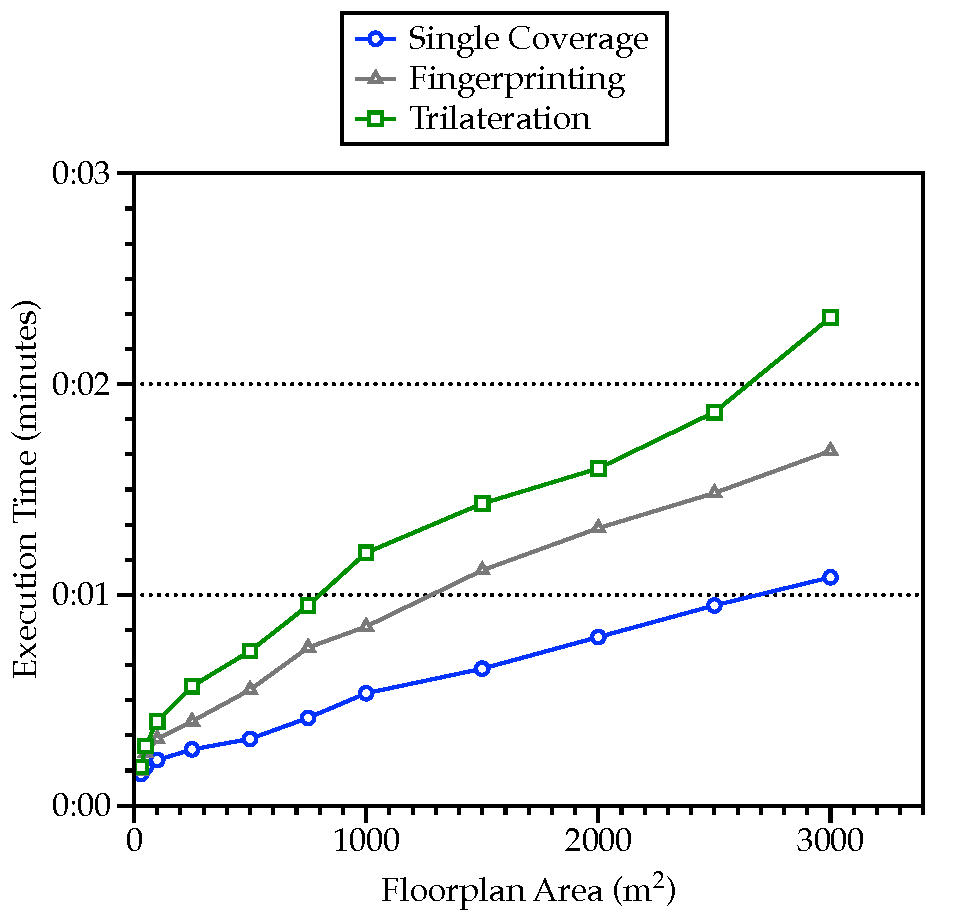
\includegraphics[scale=0.45]{exec_times.pdf}
\caption{Execution time of the tool with floor plans of different areas, for each covering technique ($R_{max} = 20$, $target = 95\%$, $r_t=8$).}
\label{fig:time}
\end{figure}
In the given example, $R_{max}$ has been fixed to 20 restarts, the $target$ coverage equals to 95\% of the total area, a single node type available with a range of 8 meters, covering floor-plans with rectangular areas. The graph shows that for single coverage, the execution time is low even for areas of 3000 squared meters. For trilateration and fingerprinting, the execution times become high from floor-plan of $2500~m^2$. However, the tests represent a bad case in which the map dimension is very large while the node range available and the spatial resolution are small (respectively 8m and 1m). Increasing the range or the resolution, the instance of the problem decrease, resulting in faster executions.

A key aspect that characterizes the goodness of the proposed approach is the improvement of the objective function achieved by the VNS algorithm with respect to the first Greedy configuration. For this test we have run the tool several times with a floor-plan area of $2500~m^2$ and a node range of $12m$. The number of reference nodes allocated is determined by the Greedy procedure and increase with $S$, while the number of VNS restarts $R_{max}$ has been fixed to 35.
\begin{figure}[h!tb]
\centering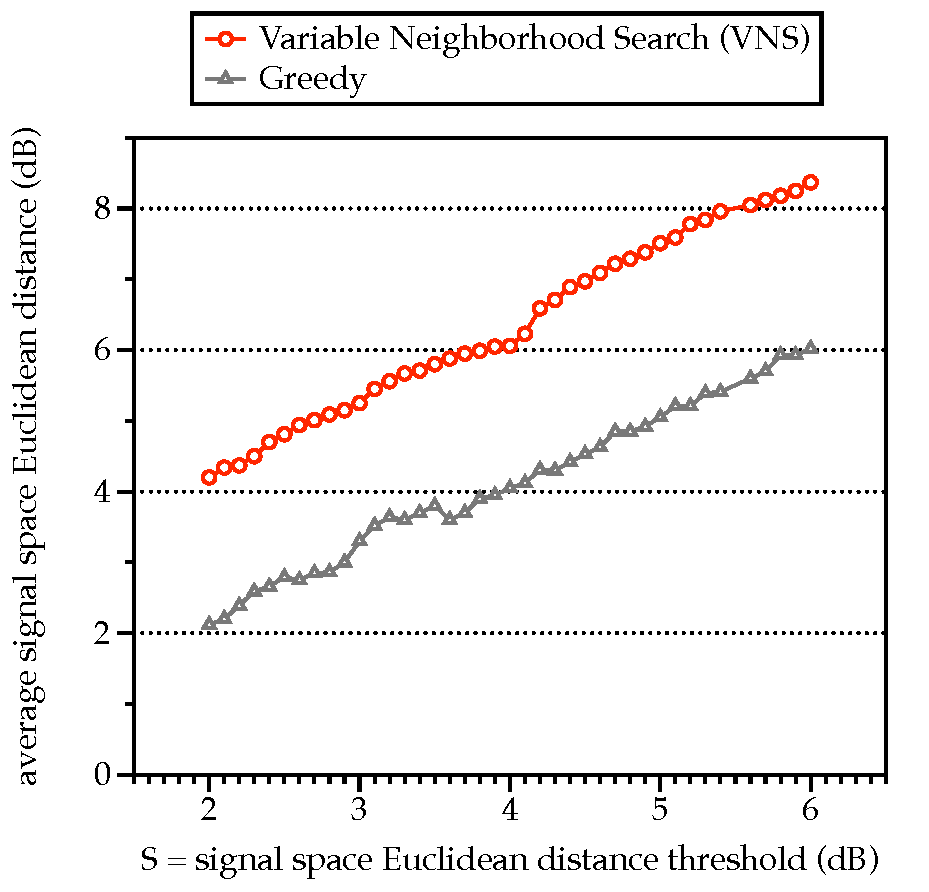
\includegraphics[scale=0.45]{greedy_vs_vns.pdf}
\caption{Average signal space Euclidean distance ($z$) obtained with the Greedy execution and compared with the $z$ value after the VNS optimization. $z$ values expressed as a function of the threshold $S$. Floor-plan area $=2500~m^2$, $R_{max} = 20$, $target = 100\%$, $r_t=12$}
\label{fig:greedy_vns}
\end{figure}
In Fig.~\ref{fig:greedy_vns} we reported the value of $z$, i.e. the average signal space Euclidean distance obtained with the first Greedy execution, compared with the $z$ value after the VNS optimization. The graph reports the $z$ values as a function of the threshold $S$, described in section~\ref{subsec:greedy} as the minimum value of average signal space Euclidean distance ($z$) required during the Greedy procedure. The graph shows that moving the threshold within the range $(2,6)$dB the VNS is able to improve the $z$ value constantly around 2 dB.
Although the VNS improvement is not astonishing for what regard the average value, Fig.~\ref{fig:greedy_vns2} shows that the variance is strongly improved. This has been achieved moving from the objective function $z$ used in Greedy procedure to the $Z$ function of the VNS. The $Z$ objective function has in fact the purpose to provide as many target location as possible with a high signal space Euclidean distance w.r.t. the surrounding locations.

\begin{figure}[h!tb]
\centering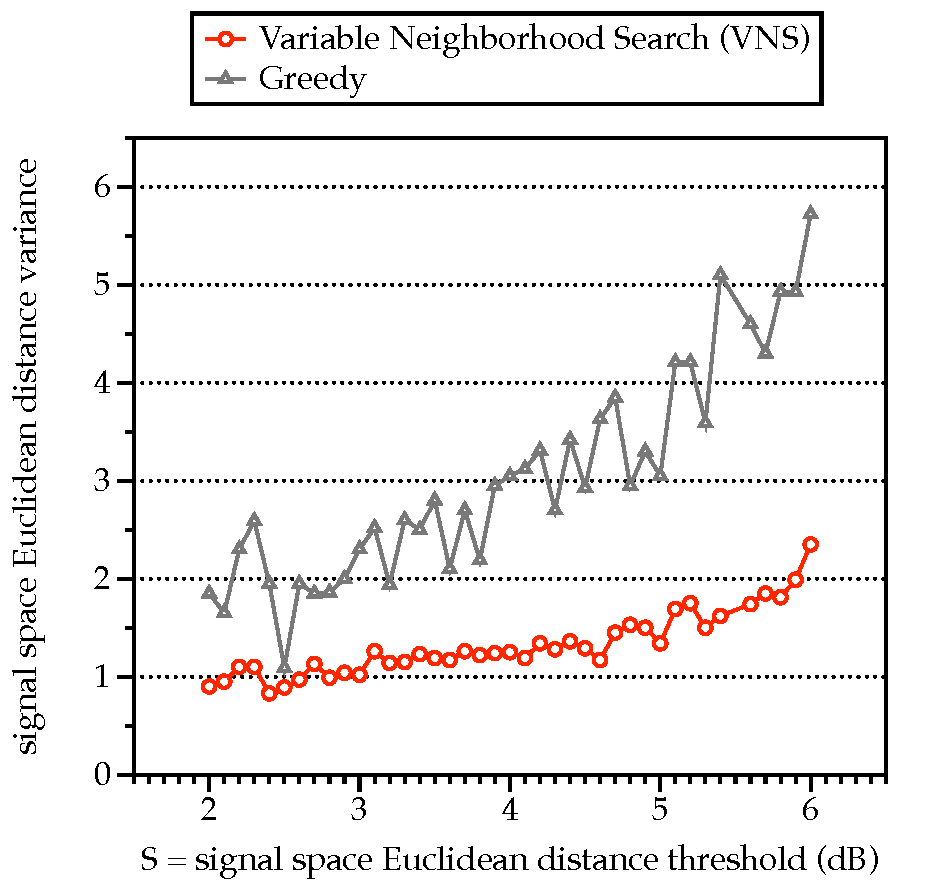
\includegraphics[scale=0.45]{greedy_vs_vns2.pdf}
\caption{Signal space Euclidean distance variance obtained with the Greedy execution and compared with the $z$ value after the VNS optimization. Values expressed as a function of the threshold $S$. Floor-plan area $=2500~m^2$, $R_{max} = 20$, $target = 100\%$, $r_t=12$}
\label{fig:greedy_vns2}
\end{figure}

\begin{figure}
\centering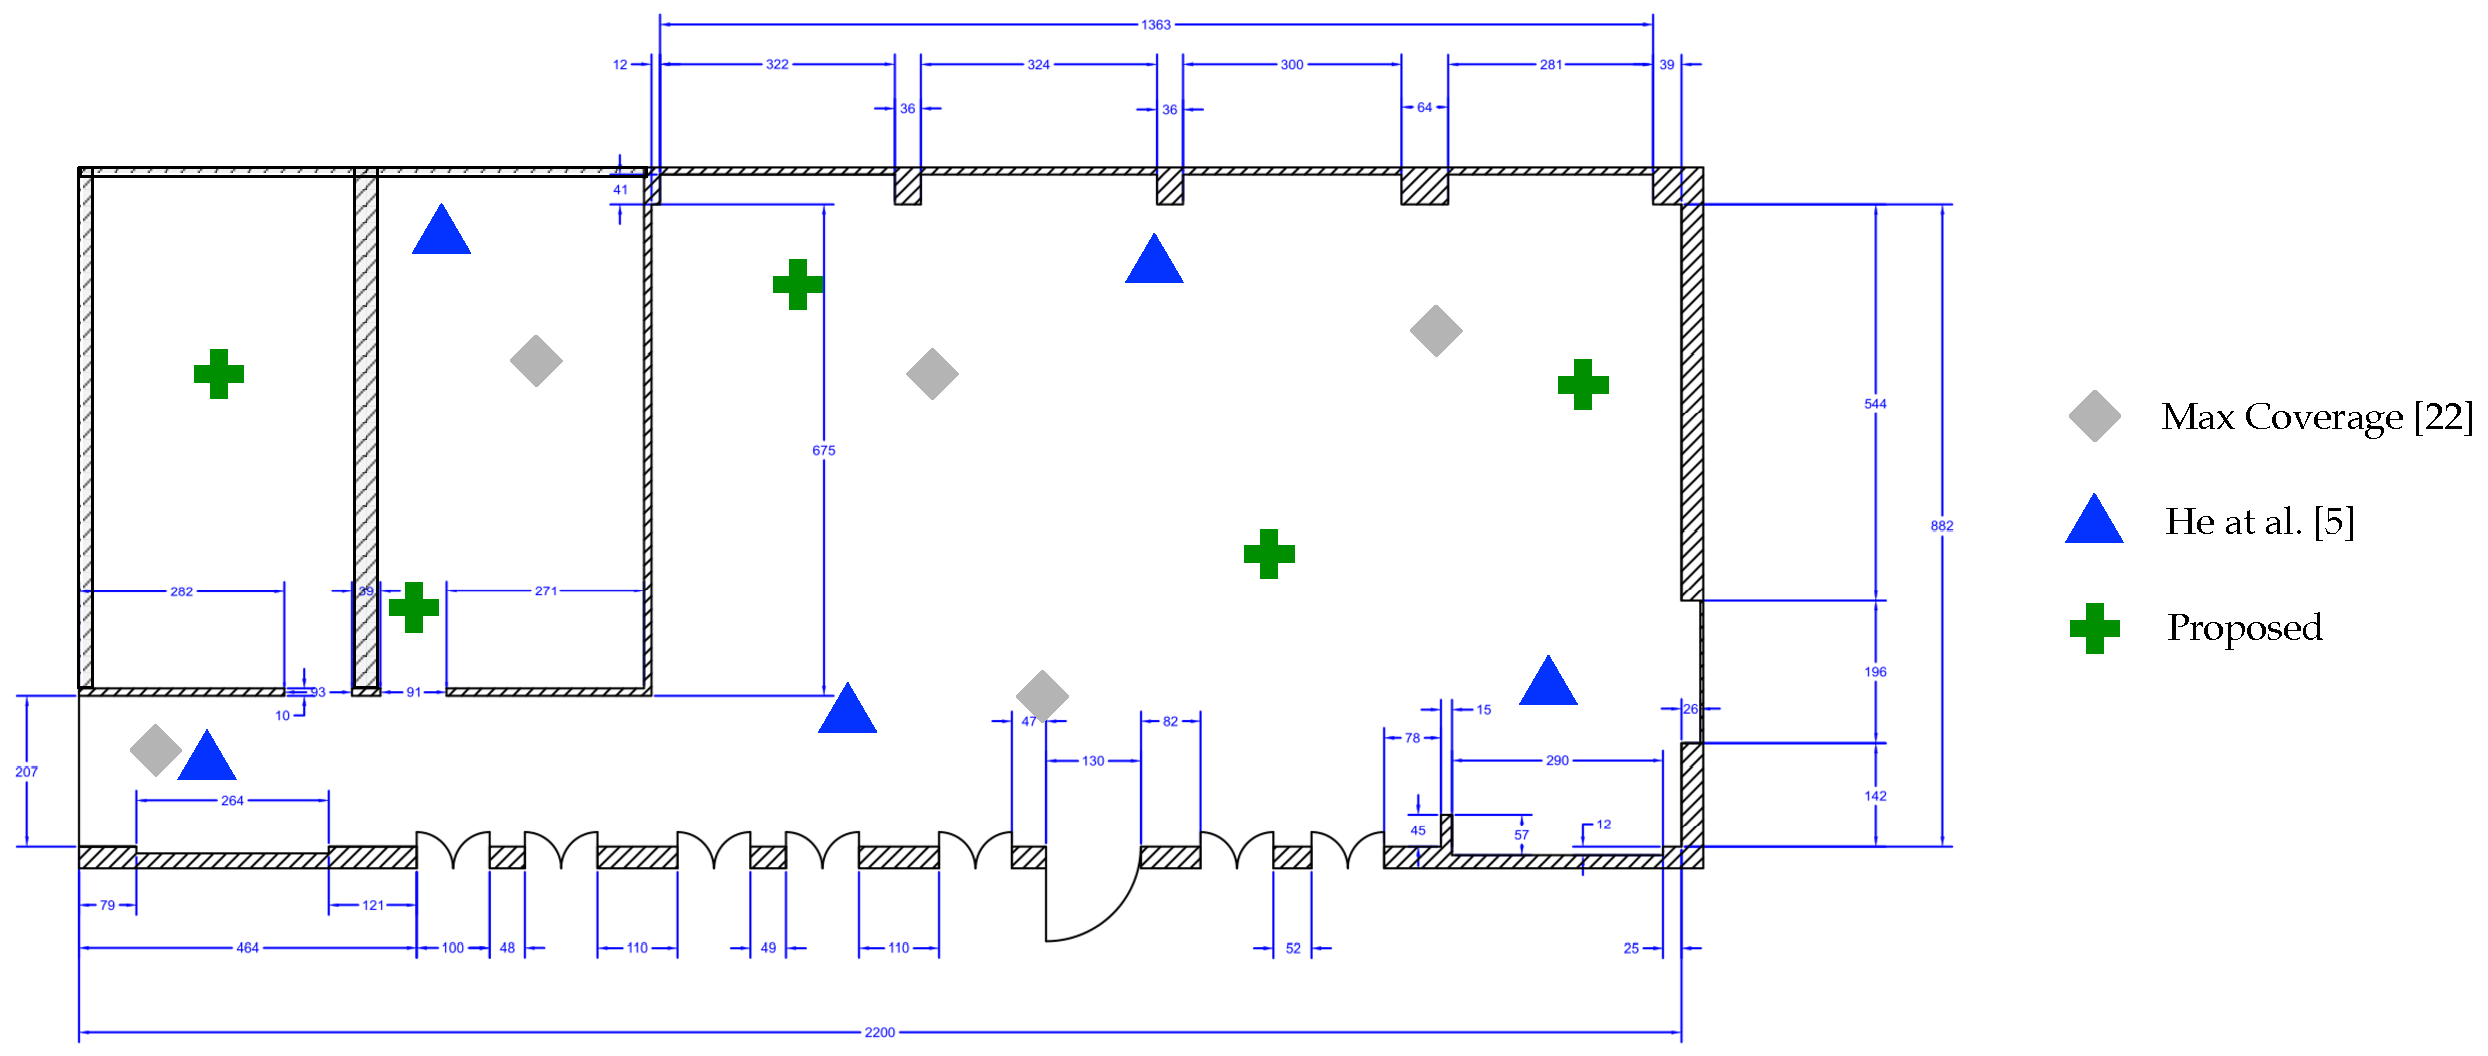
\includegraphics[scale=0.37]{necst.pdf}
\caption[NECST Lab floor-plan used as indoor environment testbed for deployments evaluation.]{NECST Lab floor-plan, located at the basement of DEIB department at Politecnico di Milano. Each allocation corresponds to a BLE beacon with a range of 7 meters. Green crosses indicates allocations provided by our algorithm, gray rhombus represent allocations from \cite{He2011} while blue triangle positions have been computed maximizing the coverage \cite{Kouakou2010a}.}
\label{fig:necst}
\end{figure}

\subsection{Experimental Setup and Accuracy Evaluation}
The proposed tool was evaluated using data collected from a real-world environment, the NECST Lab, located at the basement of DEIB department at Politecnico di Milano. The dimension of the test-bed is 198 squared meters ($9x22m$). We collected Bluetooth Low Energy (BLE) signal data coming from BLE beacons with a coverage radius of 7 meters. Signal data has been collected using a Nexus 5 smartphone running Android 6.0.1.
First, the NECST Lab floor-plan has been designed using our tool, obtaining the optimal number of beacons ($|N|=5$) and their allocation for fingerprinting localization. $R_{max}$ has been fixed to 20 restarts, the $target$ coverage equals to 100\% of the total area, a single node type available with a range of 7 meters, and the threshold $S=4,5$.
We collected 40 training samples for the localization algorithm using the obtained allocation. Then, the test samples were collected at distinct positions changing the phone orientation and the way in which user was keeping it, for example by hand or in a pocket. For the entire duration of training and test phase, the number of occupants and their enabled wireless devices has changed, from a minimum of 3 to a maximum of 17 people. This variation affects the accuracy performances, but at the same time contributes in obtaining realistic results. The training and test phase has been repeated with two configurations coming from different allocation algorithms: maximization of the coverage \cite{Kouakou2010a} and the allocation algorithm proposed by He at al. in \cite{He2011}. For these two algorithms, the number of employed nodes has been fixed to 5.
KNN with $K=3$ has been employed as the fingerprinting algorithm.

\begin{figure}[h!tb]
\centering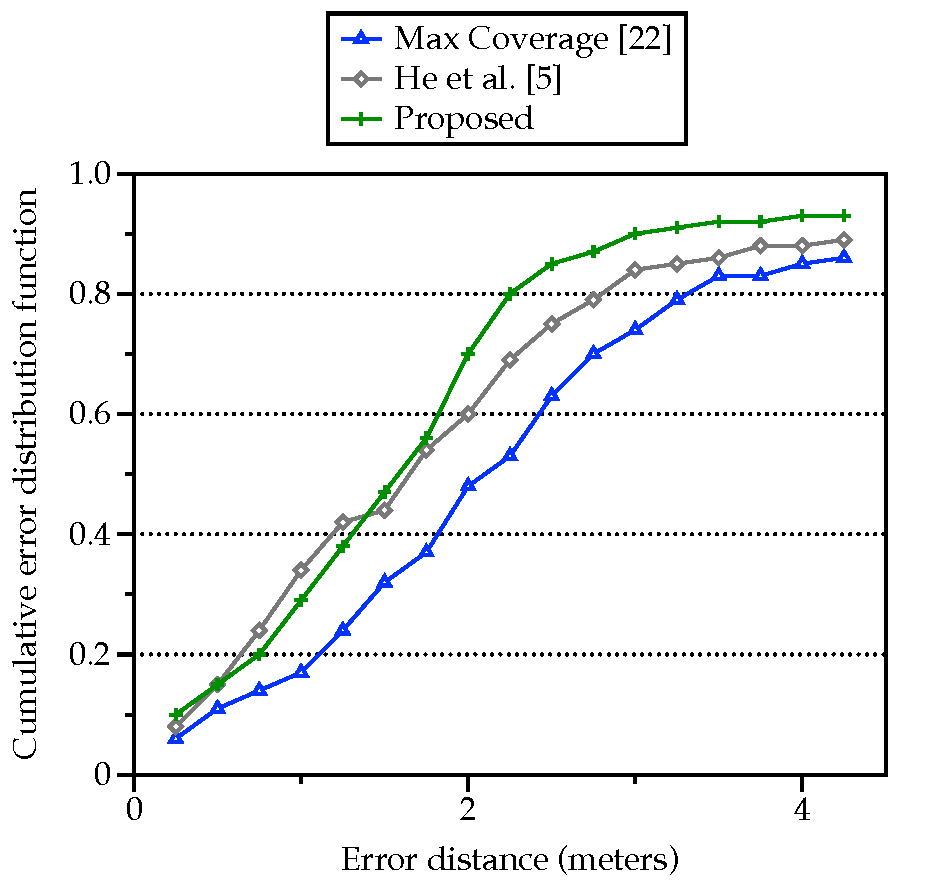
\includegraphics[scale=0.45]{loc_error.pdf}
\caption{Cumulative error distribution function experienced by our approach ad compared with two different solutions from the state-of-the-art.}
\label{fig:loc_error}
\end{figure}

A first result is showed in figure \ref{fig:loc_error}. The cumulative error distribution function shows that from 1.5 meters our approach performs better. Under 1.5 meters, He at al. approach performs better, but the difference in accuracy is marginal.

\begin{figure}[h!tb]
\centering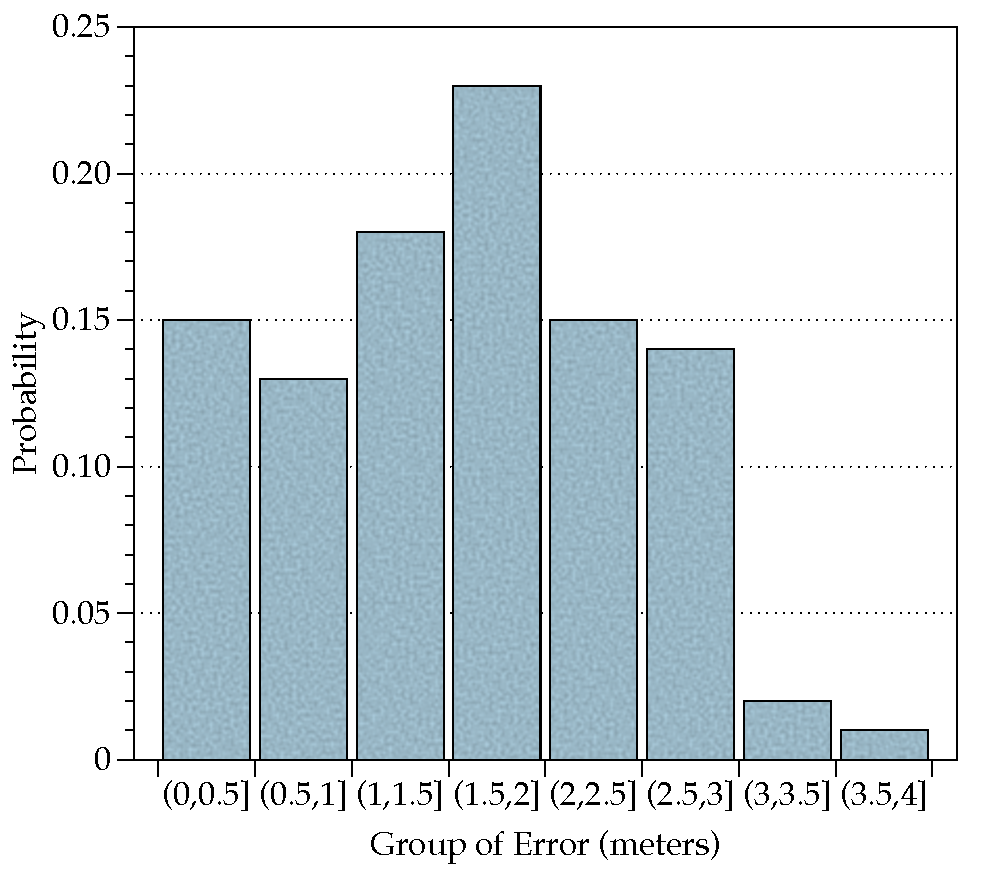
\includegraphics[scale=0.45]{group_errors.pdf}
\caption{Mean positioning accuracy of the proposed allocation algorithm divided into different error ranges.}
\label{fig:group_errors}
\end{figure}

Figure~\ref{fig:group_errors} shows the mean positioning accuracy divided into different error ranges: $( 0,0.5],$ $(0.5,1],$ $(1,1.5],$ $(1.5,2],$ $(2,2.5],$ $(2.5,3],$ $(3,3.5],$ $(3.5,4]$. It's possible to notice that the majority of the localization errors appears within the $(1.5,2]$ meters.
The test-bed floor-plan, composed by 3 rooms, has been reported in figure \ref{fig:necst}. Green crosses indicates allocations provided by our algorithm, gray rhombus represent allocations from \cite{He2011} while blue triangle positions have been computed maximizing the coverage \cite{Kouakou2010a}.

\subsection{Cost-effectiveness Analysis}
A feature of our tool interesting for testing is the possibility to obtain solutions from mixed node types, with different characteristics and costs. In particular, given two types $t_1$ and $t_2$ characterized by two ranges $r_i$, and two costs $c_i$, it's possible to compare the total cost of a homogeneous solution with the cost of a mixed solution. Given a baseline type of node with a range $r_1=8~m$ and a cost of $c_1=60~\$$, we can assume the presence on the market of a second type of hardware, with the half of the range distance ($r_2=4~m$). The area covered by $t_1$ ($\approx200~m^2$) is four times bigger than the coverage of $t_2$ ($\approx50~m^2$). In order to obtain a fair test, the cost of $t_2$ should be \(c_2 \geq c_1/4\), and so we set $c_2=20~\$$. This test has been performed with a $target$ coverage of 95\% on a rectangular map of $1000~m^2$.

From Table \ref{tab:costs} it's possible to observe that, although hardware nodes of type $t_2$ have a lower convenience in terms of $\frac{area}{price}$ ($t_1$ outperform $t_2$ in homogeneous solutions), the mixed strategy can use the smaller range nodes to reduce the total cost. 
\begin{table}[h!tb]
  \centering
  \renewcommand{\arraystretch}{1.5}
  \caption{Cost of homogeneous and mixed solutions ($A=1000~m^2$, $target=95\%$, $r_1=8m$, $r_2=4m$, $c_1=60\$$, $c_2=20\$$).}
  \label{tab:costs}
  \begin{tabular}{|c|c|c|c|}
    \hline
    \multirow{2}{*}{\textbf{Node types}} & \multicolumn{3}{c|}{\textbf{Solution Costs (in \$)}}\\
    \cline{2-4}
    & Single & Trilateration & Fingerprinting\\
    \hline
    $T=\{t_1\}$ & 480 & 1440 & 840\\
    $T=\{t_2\}$ & 500 & 1620 & 880\\
    $T=\{t_1, t_2\}$ & 440 & 1280 & 760\\ \hline
  \end{tabular}
\end{table}
This because less powerful nodes of type $t_2$ are employed to cover small portions of the floor-plan, like corners or small regions left uncovered by the larger range nodes.

The amount of saving in the total cost of the mixed solution doesn't depend only on the nodes range and price, but also on the irregularity of the floor plan perimeter. A distinguish feature of the proposed tool respect to other works is the possibility to cover spaces that are not necessarily rectangular or squared. The level of irregularity of a floor plan can be identified by the minimum number of rectangles that compose the shape. In Figure \ref{fig:irregularity} for example, the index of the floor plan irregularity is $I=4$. 
\begin{figure}[h!tb]
\centering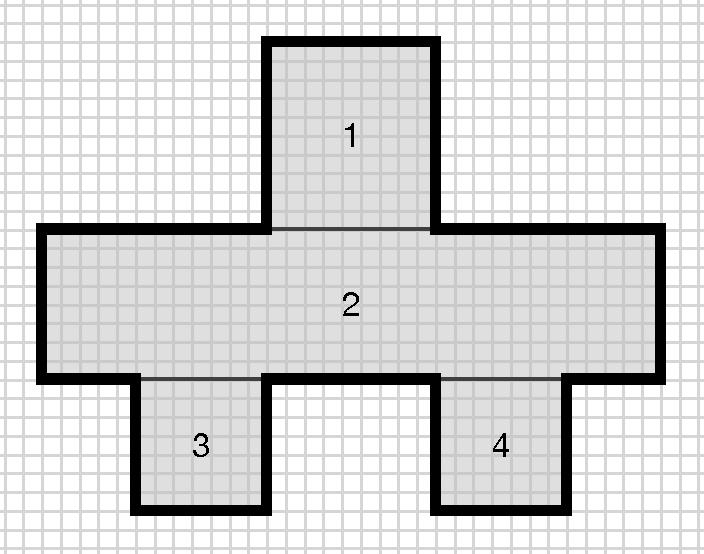
\includegraphics[scale=0.47]{irregularity.pdf}
\caption{Irregularity of the floorplan perimeter summarized by the minimum number of rectangles.}
\label{fig:irregularity}
\end{figure}
We experimented the behavior of the tool increasing the level of irregularity, while maintaining a constant total area of $1000~m^2$. The test has been done with the same nodes configuration used in table~\ref{tab:costs} (homogeneous $T=t_1$, mixed $T=t_1,t_2$). The results shown in Table~\ref{tab:irregularity} proven that increasing the floor-plan irregularity, the cost difference between homogeneous and mixed solution becomes higher. This is caused by the increasing number of corners in the map, that can be covered with less powerful nodes.
\newcolumntype{Y}{>{\centering\arraybackslash}X}
\begin{table}[H]
  \centering
  \renewcommand{\arraystretch}{1.2}
  \caption{Cost differences (in \$) between homogeneous and mixed solution increasing the floor plan irregularity (area fixed to $1000~m^2$).}
  \label{tab:irregularity}
  \begin{tabularx}{\columnwidth}{|c|YY|YY|YY|}
    \hline
    \multirow{2}{0.55cm}{\textbf{$~~I$}} & \multicolumn{2}{c|}{\textbf{Single}} & \multicolumn{2}{c|}{\textbf{Trilater.}} & \multicolumn{2}{c|}{\textbf{Fingerprint.}}\\
    \cline{2-7}
    & homog. & mixed & homog. & mixed & homog. & mixed\\
    \hline
    1 & 480 & 440 & 1440 & 1280 & 840 & 760\\
    2 & 480 & 440 & 1500 & 1320 & 840 & 780\\
    4 & 600 & 500 & 1560 & 1380 & 900 & 820\\
    8 & 720 & 580 & 1680 & 1480 & 1200 & 920\\
    \hline
  \end{tabularx}
  \end{table}
In conclusion, experimental results show that for most of the problem instances, a solution can be obtained in reasonable execution times. Depending on the available hardware types, homogeneous solutions could be improved with the employment of different type of nodes.
\section{Localization Accuracy}
\section{Responsiveness Test}
\section{Power Consumption}
\section{Stress Test}
%
% -----------------------------END------------------------------------- %